\baitracnghiem{lephulu:01}{%01}{
Hàm số $f(x)$ có đạo hàm trên $\mathbb{R}$ và ${f}'(x)<0,\forall x\in (0;3);{f}'(x)>0,\forall x\in (4,7).$ Xét
${({{x}_{1}}-{{x}_{2}})(f({{x}_{1}})   - f({{x}_{2}}))}$  với ${{x}_{1}},{{x}_{2}}\in \mathbb{R}$.
Hỏi với cặp giá trị nào sau đây thì biểu thức trên là số dương?
}{\datcot[2]\bonpa
{\sai{${{x}_{1}}=1,{{x}_{2}}=2$}}
{\sai{${{x}_{1}}=5,{{x}_{2}}=2$}}
{\sai{${{x}_{1}}=1,{{x}_{2}}=6$}}
{\dung{${{x}_{1}}=6,{{x}_{2}}=5$}}
}
\baitracnghiem{lephulu:02}{%02}{
Biết rằng $x=m$ là một điểm cực trị của hàm số $y=\dfrac{1}{2}{{x}^{4}}-\dfrac{3}{2}m{{x}^{2}}+x$. Tính giá trị của $m.$
}{\datcot[2]\bonpa
{\sai{$m=0$}}
{\sai{$m=1$}}
{\dung{$m=-\dfrac{1}{2}$}}
{\sai{$m=1\pm \sqrt{3}$}}
}
\baitracnghiem{lephulu:03}{%03}{
Một hàm số $f(x)$ xác định và có đạo hàm cấp một, cấp hai trên $\mathbb{R}$. Biết rằng $x=1$ là điểm cực tiểu và $x=10$ là điểm cực đại của hàm số. Hỏi điều nào sau đây luôn đúng?
}{\datcot[2]\bonpa
{\sai{$f(1)>f(10)$}}
{\sai{${f}'(1)>{f}'(10)$}}
{\dung{${{f}'}'(1)>{{f}'}'(10)$}}
{\sai{$f(1)<f(10)$}}
}
\baitracnghiem{lephulu:04}{%04}{
Tìm $m$ để giá trị lớn nhất của hàm số $f(x)={{x}^{2}}+2{{m}^{2}}x-16m$ ($m$ là tham số) trên đoạn $[0;2]$ là nhỏ nhất.
}{\datcot\bonpa
{\dung{$2$}}
{\sai{$3$}}
{\sai{$4$}}
{\sai{$1$}}
}
\baitracnghiem{lephulu:05}{%05}{
Hàm số $y=\dfrac{ax+b}{cx+d}$ với $ad\ne bc$ có đồ thị như hình bên. 
Hỏi khẳng định nào sau đây không thể xảy ra?
\begin{center}
\begin{tikzpicture}[thick,>=stealth,x=1cm,y=1cm,scale=.5] 
\clip(-2.5,-2.5) rectangle (4.5,4.5);
\draw[very thick,blue,smooth,samples=100,domain=1.5:4.5] plot(\x,{((\x)+1)/((\x)-1)});
\draw[very thick,blue,smooth,samples=100,domain=-2.5:0.5] plot(\x,{((\x)+1)/((\x)-1)});
\end{tikzpicture}
\end{center}
}{\datcot[2]\bonpa
{\sai{$ac>bd$}}
{\dung{$ad>bc$}}
{\sai{$ab>cd$}}
{\sai{$abcd<1$}}
}
\baitracnghiem{lephulu:06}{%06}{
Có bao nhiêu số nguyên $m$ để hàm số $y=\dfrac{20x}{\sqrt{17{{x}^{2}}-1}-m\left| x \right|}$ có $4$ đường tiệm cận (bao gồm tiệm cận đứng và tiệm cận ngang)?
}{\datcot\bonpa
{\sai{$4$}}
{\sai{$3$}}
{\sai{Vô số}}
{\dung{$5$}}
}
\baitracnghiem{lephulu:07}{%07}{
Biết đồ thị hàm số $y={{x}^{4}}-2{{x}^{2}}+m$ có ba điểm cực trị là $A,B,C.$ Tìm $m$ sao cho tam giác $ABC$ bị hai trục tọa độ $Ox,Oy$ chia thành bốn phần có diện tích bằng nhau.
}{\datcot\bonpa
{\sai{$\dfrac{1}{2}$}}
{\dung{$\dfrac{\sqrt{2}}{2}$}}
{\sai{$2$}}
{\sai{$\sqrt{2}$}}
}
\baitracnghiem{lephulu:08}{%08}{
Bốn đường tiệm cận của hai hàm số $y=\dfrac{ax}{bx+1}$ và $y=\dfrac{cx}{{\rm d}x+1}$ đôi một cắt nhau tạo thành một hình chữ nhật chứa gốc tọa độ $O$ bên trong nó. Hỏi kết luận nào sau đây luôn đúng?
}{\datcot[2]\bonpa
{\dung{$abcd<0$}}
{\sai{$a+b+c+d>0$}}
{\sai{$\dfrac{1}{b}+\dfrac{1}{d}>0$}}
{\sai{$\dfrac{a}{b}+\dfrac{c}{d}<0$}}
}
\baitracnghiem{lephulu:09}{%09}{
Cho hàm số $y=\dfrac{2x+m}{{{x}^{2}}-2x+3}$ với tham số $m$. Tìm $m$ để đường thẳng qua hai điểm cực trị của đồ thị hàm số không có điểm chung nào với góc phần tư thứ hai của mặt phẳng tọa độ $Oxy$ (cho phép có phần chung với hai trục tọa độ).
}{\datcot\bonpa
{\sai{$m\ge 2$}}
{\dung{$m\le -1$}}
{\sai{$m\ge 1$}}
{\sai{$m\le 0$}}
}
\baitracnghiem{lephulu:10}{%10}{
Ở môn Toán trong kỳ thi THPT Quốc gia, một học sinh dự định sẽ dành $40$ phút để làm $21$ câu hỏi cuối đề; gồm $14$ câu hỏi mức độ III và $7$ câu hỏi mức độ IV. Nếu học sinh này dành $x$ phút cho các câu mức độ III, tổng điểm bạn có thể đạt được cho phần này là $14\times 0,2\times f(x)$ với $f(x)=\dfrac{x}{x+1}$. Còn ở mức độ IV, tổng đó sẽ là $7\times 0,2\times g(x)$ với $g(x)=\dfrac{2x}{3x+1}.$ Hỏi tổng điểm bạn này đạt được cho hai phần này lớn nhất là bao nhiêu? (làm tròn đến 1 chữ số thập phân)
}{\datcot\bonpa
{\sai{$3,0$}}
{\dung{$3,6$}}
{\sai{$4,2$}}
{\sai{$3,8$}}
}
\baitracnghiem{lephulu:11}{%11}{
Cho hàm số $y=\dfrac{1}{5}(m-1){{x}^{5}}+\dfrac{1}{2}(m+1){{x}^{2}}+(3m-3)x$ với tham số $m$ có đồ thị $(C).$ Biết rằng tồn tại hai điểm $A,B\in (C)$ mà tiếp tuyến của $(C)$ tại $A,B$ vuông góc với nhau, khi đó
}{\datcot[2]\bonpa
{\sai{$\dfrac{1}{2}<m<2$}}
{\dung{$\dfrac{3}{5}\le m\le \dfrac{5}{3}$}}
{\sai{$-1\le m\le 0$}}
{\sai{$1\le m\le 5$}}
}
\baitracnghiem{lephulu:12}{%12}{
Số nguyên dương nhỏ nhất thuộc tập xác định của $y={{\log }_{2}}({{\log }_{2}}({{\log }_{2}}({{\log }_{2}}({{\log }_{2}}x))))$ là
}{\datcot\bonpa
{\sai{$1$}}
{\sai{${{2}^{5}}$}}
{\dung{$17$}}
{\sai{${{2}^{{{2}^{{{2}^{2}}}}}}+1$}}
}
\baitracnghiem{lephulu:13}{%13}{
Biết rằng nếu $a,b,c$ lập thành cấp số cộng thì $a+c=2b$; còn nếu $a,b,c$ lập thành cấp số nhân thì $ac={{b}^{2}}$. Với các số thực dương $x,y$, ta có các số $2,{{4}^{4}},{{8}^{y}}$ lập thành cấp số nhân và các số${{\log }_{2}}y,{{\log }_{2}}x,{{\log }_{2}}45$ lập thành cấp số cộng. Tìm $x.$ 
}{\datcot[2]\bonpa
{\dung{$x=15$}}
{\sai{$x=\sqrt{105}$}}
{\sai{$x=225$}}
{\sai{$x=105$}}
}
\baitracnghiem{lephulu:14}{%14}{
Với mọi giá trị của $a>0,a\ne 1$, đồ thị hàm số $y={{a}^{x-3}}$ luôn đi qua điểm cố định $A$ và đồ thị hàm số $y={{\log }_{a}}(5-x)$ luôn đi qua điểm cố định $B.$ Tính khoảng cách $AB.$ 
}{\datcot\bonpa
{\sai{$1$}}
{\sai{$2$}}
{\dung{$\sqrt{2}$}}
{\sai{$\dfrac{1}{2}$}}
}
\baitracnghiem{lephulu:15}{%15}{
Xét hàm số $f(x)={{e}^{x}}(a\sin x+b\cos x)$ với $a,b$ là tham số. Biết rằng tồn tại $x\in \mathbb{R}$ để $f(x)+{{f}'}'(x)=5{{e}^{x}}$. Khi đó, nhận xét nào sau đây là đúng?
}{\datcot[2]\bonpa
{\sai{$a+b=5$}}
{\dung{${{a}^{2}}+{{b}^{2}}\ge 5$}}
{\sai{$\left| a-b \right|\le 5$}}
{\sai{${{a}^{2}}+{{b}^{2}}=25$}}
}
\baitracnghiem{lephulu:16}{%16}{
Cho phương trình ${{4}^{x}}-(10m+1)\cdot {{2}^{x}}+32=0$. Biết rằng phương trình này có hai nghiệm là ${{x}_{1}},{{x}_{2}}$ thỏa mãn $\dfrac{1}{{{x}_{1}}}+\dfrac{1}{{{x}_{2}}}+\dfrac{1}{{{x}_{1}}{{x}_{2}}}=1$. Khi đó, khẳng định nào sau đây về $m$ là đúng?
}{\datcot[2]\bonpa
{\sai{$0<m<1$}}
{\dung{$1<m<2$}}
{\sai{$2<m<3$}}
{\sai{$-1<m<0$}}
}
\baitracnghiem{lephulu:17}{%17}{
Một tam giác vuông có độ dài hai cạnh góc vuông là $\sqrt{{{\log }_{2}}x},\sqrt{{{\log }_{2}}(64x)}$. Biết rằng đường cao ứng với cạnh huyền của tam giác có độ dài là $2$, tìm $x.$ 
}{\datcot\bonpa
{\sai{$x=12$}}
{\sai{$x=2$}}
{\dung{$x=64$}}
{\sai{$x=6$}}
}
\baitracnghiem{lephulu:18}{%18}{
Hệ cơ số $m-$ phân là hệ thống tính toán, biểu diễn số chỉ dùng $m$ “chữ số” (nếu $m>10$ thì cần mượn thêm các chữ cái). Một số nguyên dương $n$ trong hệ thập phân, khi viết trong hệ $m-$phân sẽ có $\left[ {{\log }_{m}}n \right]+1$ chữ số ($[x]$ chỉ số nguyên lớn nhất không vượt quá $x$). Câu toán đặt ra là với hai số nguyên dương $a,b>1,$ số ${{a}^{b}}{{a}^{a}}-1$ viết trong hệ $a$ phân có $19$ chữ số, còn số ${{({{b}^{a}})}^{b}}-1$ viết trong hệ $b$ phân có $88$ chữ số; hỏi $2017$ viết trong hệ $\left| a-b \right|-$phân có mấy chữ số?
}{\datcot\bonpa
{\sai{$5$}}
{\sai{$6$}}
{\dung{$7$}}
{\sai{$8$}}
}
\baitracnghiem{lephulu:19}{%19}{
Tìm $m$ nhỏ nhất để hàm số $y=2\ln \left( x+\sqrt{1+{{x}^{2}}} \right)+{{x}^{3}}-mx$ nghịch biến trên $\left( -1;\sqrt{3} \right)$.
}{\datcot[2]\bonpa
{\dung{$m=10$}}
{\sai{$m=3+\sqrt{2}$}}
{\sai{$m=2$}}
{\sai{$m=2\ln 2$}}
}
\baitracnghiem{lephulu:20}{%20}{
Tìm $m$ để BPT $\dfrac{{{\log }_{2}}(mx)}{{{\log }_{2}}(1-x)}+\dfrac{{{\log }_{2}}(m-mx)}{{{\log }_{2}}x}\le -1$ có nghiệm duy nhất $x\in (0;1)$?
}{\datcot\bonpa
{\sai{$2$}}
{\sai{$\sqrt{2}$}}
{\dung{$2\sqrt{2}$}}
{\sai{$4$}}
}
\baitracnghiem{lephulu:21}{%21}{
Với $a,b,c$ là các số thực lớn hơn $1$, đặt $x={{\log }_{a}}(bc),y={{\log }_{b}}(ca),z={{\log }_{c}}(ab).$ Tìm giá trị nhỏ nhất của biểu thức $P=x+y+4z.$ 
}{\datcot\bonpa
{\sai{$6$}}
{\sai{$12$}}
{\dung{$10$}}
{\sai{$16$}}
}
\baitracnghiem{lephulu:22}{%22}{
Cho hàm số $f(x)$ liên tục trên $\mathbb{R}$ thỏa mãn $\displaystyle\int_{0}^{6}{f(x){\rm d}x}=6,\displaystyle\int_{3}^{10}{f(x)}{\rm d}x=4,\displaystyle\int_{3}^{6}{f(x)}{\rm d}x=1.$ Tính giá trị của $I=\displaystyle\int_{0}^{10}{f(x){\rm d}x}$.
}{\datcot\bonpa
{\sai{$3$}}
{\sai{$10$}}
{\dung{$9$}}
{\sai{$8$}}
}
\baitracnghiem{lephulu:23}{%23}{
Tìm $a$ để tích phân sau đây tồn tại $\displaystyle\int_{1}^{1+a}{\dfrac{{\rm d}x}{x(x-3)(x-4)}}$:
}{\datcot[2]\bonpa
{\sai{$a<2$}}
{\sai{$a\ne 2,a\ne 3$}}
{\dung{$-1<a<2$}}
{\sai{$a<3$}}
}
\baitracnghiem{lephulu:24}{%24}{
Biết rằng $\displaystyle\int_{0}^{{{\pi }^{2}}}{\left( \sin \sqrt{x}+\cos \sqrt{x} \right){\rm d}x}=A+B\pi $. Tính $A+B.$ 
}{\datcot\bonpa
{\sai{$2$}}
{\sai{$-4$}}
{\dung{$-2$}}
{\sai{$\pi $}}
}
\baitracnghiem{lephulu:25}{%25}{
Hai người $A,B$ đang chạy xe ngược chiều nhau thì xảy ra va chạm, hai xe tiếp tục di chuyển thêm được một quãng đường nữa thì dừng hẵn. Biết rằng ngay sau khi va chạm, một người di chuyển tiếp với vận tốc ${{v}_{1}}(t)=6-2t,$ người còn lại di chuyển với vận tốc ${{v}_{2}}(t)=8-4t$. Tính khoảng cách hai xe khi đã dừng hẵn.
\begin{center}
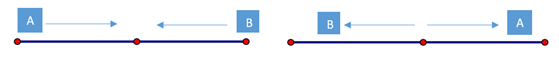
\includegraphics[scale=.6]{lephuclul225}
\end{center}
}{\datcot\bonpa
{\sai{$16m$}}
{\dung{$17m$}}
{\sai{$12m$}}
{\sai{$15m$}}
}
\baitracnghiem{lephulu:26}{%26}{
Cho đồ thị của hàm số $y={{x}^{3}}$ trên $[0;1]$ và một số thực $t\in [0;1].$ Gọi ${{S}_{1}}$ là diện tích hình giới hạn bởi các đường $x=0,y={{x}^{3}},y={{t}^{3}}$ ; ${{S}_{2}}$ là diện tích hình giới hạn bởi các đường $y={{x}^{3}},y={{t}^{3}},x=1$. Gọi $m,M$ là giá trị nhỏ nhất, lớn nhất của ${{S}_{1}}+{{S}_{2}}.$ Tính $2M+16m.$ 
}{\datcot\bonpa
{\sai{$3$}}
{\dung{$5$}}
{\sai{$7$}}
{\sai{$1$}}
}
\baitracnghiem{lephulu:27}{%27}{
Cho hai hàm số $f(x)$ và $g(x)$ liên tục, có đạo hàm trên $\mathbb{R}$ và thỏa mãn ${f}'(0){f}'(1)\ne 0$ và$g(x){f}'(x)=x(x-1){{e}^{x}}$ với mọi $x$. Tính giá trị của tích phân  ${I=\displaystyle\int_{0}^{1}{f(x){g}'(x){\rm d}x}}$.
}{\datcot\bonpa
{\sai{$2-e$}}
{\sai{$e$}}
{\sai{$2e$}}
{\dung{$3-e$}}
}
\baitracnghiem{lephulu:28}{%28}{
Trên mặt bàn, có một cái bánh kem hình chuông úp ngược. Mỗi lát cắt của bánh song song với mặt bàn đều là hình tròn, lát cắt dọc đi qua đỉnh bánh có dạng đồ thị của một parabol. Người ta muốn cắt ngang cái bánh để chia nó thành hai phần có thể tích bằng nhau. Biết rằng bánh cao $36cm$ và bán kính đường tròn đáy là $6cm.$ Hỏi nhát cắt cần tìm có độ cao $h$ so với mặt bàn là bao nhiêu?
\begin{center}
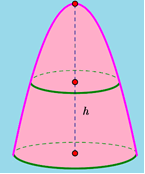
\includegraphics[scale=0.8]{lephuclul228}
\end{center}
}{\datcot[2]\bonpa
{\sai{$h=18-4\sqrt{2}$}}
{\sai{$h=18$}}
{\sai{$h=9\sqrt{2}$}}
{\dung{$h=18(2-\sqrt{2})$}}
}
\baitracnghiem{lephulu:29}{%29}{
Với hai số phức ${{z}_{1}},{{z}_{2}}$, ta gọi $A,B$ là điểm biểu diễn của ${{z}_{1}},\overline{{{z}_{1}}}$ và $C,D$ là điểm biểu diễn của ${{z}_{2}},\overline{{{z}_{2}}}$. Giả sử cả bốn điểm đều phân biệt thì $A,B,C,D$ luôn tạo thành hình gì?
}{\datcot[2]\bonpa
{\sai{Hình vuông}}
{\sai{Hình chữ nhật}}
{\sai{Hình bình hành}}
{\dung{Hình thang cân}}
}
\baitracnghiem{lephulu:30}{%30}{
Biết rằng phương trình ${{z}^{2}}+mz+4-2i=0$ có một nghiệm thuần ảo với $m\in \mathbb{R}$ và $m>0.$ Tìm nghiệm còn lại của phương trình.
}{\datcot\bonpa
{\sai{$2-i$}}
{\dung{$-1-2i$}}
{\sai{$2i$}}
{\sai{$-4i-2$}}
}
\baitracnghiem{lephulu:31}{%31}{
Cho hai số phức ${{z}_{1}},{{z}_{2}}$ thỏa mãn $\left| {{z}_{1}} \right|{{z}_{1}}=9\left| {{z}_{2}} \right|{{z}_{2}}$ và nếu gọi $M,N$ là điểm biểu diễn ${{z}_{1}},\overline{{{z}_{2}}}$ trong mặt phẳng tọa độ thì tam giác $MON$ có diện tích là $6.$ Tìm giá trị nhỏ nhất của $\left| {{z}_{1}}+{{z}_{2}} \right|.$
}{\datcot\bonpa
{\dung{$8$}}
{\sai{$6$}}
{\sai{$4\sqrt{2}$}}
{\sai{$3\sqrt{2}$}}
}
\baitracnghiem{lephulu:32}{%32}{
Trong mặt phẳng tọa độ $Oxy$, gọi $H$ là phần mặt phẳng chứa các điểm biểu diễn số phức $z$ thỏa mãn $\dfrac{z}{40}$ và $\dfrac{40}{{\bar{z}}}$ có phần thực và phần ảo đều thuộc $[0;1].$ Tính diện tích của $H.$ 
}{\datcot[2]\bonpa
{\sai{$1600$}}
{\sai{$400\pi $}}
{\sai{$50(3-\pi )$}}
{\dung{$200(6-\pi )$}}
}
\baitracnghiem{lephulu:33}{%33}{
Cho số phức $z=a+bi$ với $\left| z \right|=5$ và $b>0$ sao cho $\left| (1+2i){{z}^{3}}-{{z}^{5}} \right|$ là lớn nhất. Đặt ${{z}^{4}}=c+di$, tính tổng $c+d.$ 
}{\datcot\bonpa
{\sai{$100$}}
{\sai{$85$}}
{\dung{$125$}}
{\sai{$52$}}
}
\baitracnghiem{lephulu:34}{%34}{
Cho hai số phức ${{z}_{1}},{{z}_{2}}$ thỏa mãn $\left| {{z}_{1}} \right|=2,\left| {{z}_{2}} \right|=\sqrt{3}$ và nếu gọi $M,N$ lần lượt là điểm biểu diễn của ${{z}_{1}},i{{z}_{2}}$ thì $\widehat{MON}=30^\circ $. Tính $\left| z_{1}^{2}+4z_{2}^{2} \right|$.
}{\datcot\bonpa
{\sai{$\sqrt{5}$}}
{\dung{$4\sqrt{7}$}}
{\sai{$3\sqrt{3}$}}
{\sai{$5\sqrt{2}$}}
}
\baitracnghiem{lephulu:35}{%35}{
Cho tứ diện $ABCD$ có thể tích $V$ với $M,N$ lần lượt là trung điểm $AB,CD.$ Gọi ${{V}_{1}},{{V}_{2}}$ lần lượt là thể tích của $MNBC$ và $MNDA.$ Tính tỉ lệ $\dfrac{{{V}_{1}}+{{V}_{2}}}{V}.$ 
}{\datcot\bonpa
{\sai{$1$ }}
{\dung{$\dfrac{1}{2}$}}
{\sai{$\dfrac{1}{3}$}}
{\sai{$\dfrac{2}{3}$}}
}
\baitracnghiem{lephulu:36}{%36}{
Một hình lập phương có thể tích gấp $24$ lần thể tích một hình tứ diện đều. Hỏi cạnh hình lập phương gấp mấy lần cạnh tứ diện?
}{\datcot\bonpa
{\sai{$2\sqrt{2}$}}
{\sai{$2$}}
{\dung{$\sqrt{2}$}}
{\sai{$1$}}
}
\baitracnghiem{lephulu:37}{%37}{
Cho hình chóp tứ giác $S.ABCD$ có đáy $ABCD$ là tứ giác lồi và góc tạo bởi $(SAB),(SBC),(SCD),(SDA)$ với mặt đáy lần lượt là $90{}^\circ ,60{}^\circ ,60{}^\circ ,60{}^\circ .$ Biết rằng tam giác $SAB$ vuông cân tại $S$ có $AB=a$ và chu vi tứ giác $ABCD$ là $9a.$ Tính thể tích hình chóp $S.ABCD.$ 
}{\datcot\bonpa
{\sai{${{a}^{3}}\sqrt{3}$}}
{\sai{${{a}^{3}}\dfrac{\sqrt{3}}{4}$}}
{\dung{${{a}^{3}}\dfrac{2\sqrt{3}}{9}$ }}
{\sai{${{a}^{3}}\dfrac{\sqrt{3}}{9}$}}
}
\baitracnghiem{lephulu:38}{%38}{
Có một cái bể hình trụ cao $10dm$ với bán kính đáy $4dm$ chứa đầy nước bị một thùng gỗ hình lập phương đóng kín rơi vào làm cho một lượng nước $V$ tràn ra. Biết rằng cạnh thùng gỗ là $8dm$ và khi nó rơi vào miệng bể, một đường chéo dài nhất của nó vuông góc với mặt bể, ba cạnh của thùng chạm vào thành của bể như hình vẽ. Tính $V.$ 
\begin{center}
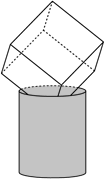
\includegraphics[scale=.7]{lephuclul238}
\end{center}
}{\datcot\bonpa
{\sai{$16\sqrt{3}$ }}
{\sai{$\dfrac{256}{9}$}}
{\sai{$\dfrac{16}{3}\sqrt{6}$}}
{\dung{$8\sqrt{6}$}}
}
\baitracnghiem{lephulu:39}{%39}{
Cho hình chóp $S.ABC$ có $SA\bot (ABC)$ và $SA=a\sqrt{2},\widehat{BAC}=45{}^\circ $. Biết rằng bán kính mặt cầu ngoại tiếp hình chóp là $a.$ Tính độ dài $BC.$ 
}{\datcot[2]\bonpa
{\dung{$BC=a$}}
{\sai{$BC=a\sqrt{2}$}}
{\sai{$BC=\dfrac{a}{\sqrt{2}}$}}
{\sai{$BC=2a$}}
}
\baitracnghiem{lephulu:40}{%40}{
Có hai mặt phẳng $(P),(Q)$ song song với nhau cắt một mặt cầu $(O,R)$ tạo thành hai hình tròn cùng bán kính. Xét hình nón có đỉnh trùng với tâm của một trong hai hình tròn, đáy trùng với hình tròn còn lại. Tính khoảng cách giữa $(P),(Q)$ để diện tích xung quanh của hình nón là lớn nhất.
}{\datcot\bonpa
{\sai{$R\sqrt{2}$}}
{\sai{$R$}}
{\dung{$\dfrac{2R\sqrt{3}}{3}$}}
{\sai{$2R\sqrt{3}$}}
}
\baitracnghiem{lephulu:41}{%41}{
Có một mảnh bìa hình chữ nhật $ABCD$ với $AB=2a,AD=4a.$ Người ta đánh dấu $E$ là trung điểm $BC$ và $F$ là điểm thuộc $AD$ sao cho $AF=a.$ Sau đó, người ta cuốn mảnh bìa lại sao cho cạnh $DC$ trùng với cạnh $AB$ tạo thành một hình trụ. Tính thể tích của tứ diện $ABEF$ với các đỉnh $A,B,E,F$ nằm trên hình trụ vừa tạo thành.
\begin{center}
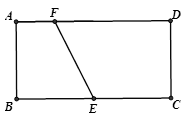
\includegraphics[scale=1.]{lephuclul241}
\end{center}
}{\datcot\bonpa
{\sai{$\dfrac{{{a}^{3}}}{3\pi }$}}
{\sai{$\dfrac{8{{a}^{3}}}{{{\pi }^{2}}}$}}
{\dung{$\dfrac{8{{a}^{3}}}{3{{\pi }^{2}}}$}}
{\sai{$\dfrac{16{{a}^{3}}}{3{{\pi }^{2}}}$}}
}
\baitracnghiem{lephulu:42}{%42}{
Cho tam giác nhọn $ABC$. Khi quay tam giác $ABC$ xung quanh các cạnh $BC,CA,AB$, ta lần lượt được các hình tròn xoay có thể tích là $\dfrac{3136}{5},\dfrac{9408}{13},672$. Tính diện tích tam giác $ABC.$
}{\datcot\bonpa
{\dung{$84$}}
{\sai{$91$}}
{\sai{$336$}}
{\sai{$1295$}}
}
\baitracnghiem{lephulu:43}{%43}{
Trong không gian với hệ trục tọa độ $Oxyz,$ cho hai điểm $A(a,b,c)$ và $B(d,e,f)$. Điều kiện để $A,B$ nằm về hai phía của mặt phẳng $(Oxy)$ là?
}{\datcot[2]\bonpa
{\sai{$ad<0$}}
{\sai{$be<0$ }}
{\dung{$cf<0$}}
{\sai{$a+d<0$}}
}
\baitracnghiem{lephulu:44}{%44}{
Trong không gian với hệ trục tọa độ $Oxyz,$ cho các điểm $A,B,C$ với $M(1;-2;2)$ là trung điểm $BC.$ Biết $\overrightarrow{AB}=(0;1;-2),\overrightarrow{AC}=(-2;-1;0).$ Tìm tọa độ điểm $A.$ 
}{\datcot[2]\bonpa
{\sai{$A(-2;2;-3)$}}
{\sai{$A(-1;1;-2)$}}
{\dung{$A(2;-2;3)$}}
{\sai{$A(0;2;-3)$}}
}
\baitracnghiem{lephulu:45}{%45}{
Trong không gian với hệ trục $Oxyz,$ xét mặt cầu $(S):{{x}^{2}}+{{(y-1)}^{2}}+{{(z-2)}^{2}}=5$ tâm $I$. Các mặt phẳng vuông góc với $OI$ và tiếp xúc với $(S)$ không đi qua điểm nào trong các điểm sau?
}{\datcot[2]\bonpa
{\sai{$(0;0;0)$}}
{\sai{$(4;-2;1)$}}
{\sai{$(1;4;3)$}}
{\dung{$(12;-1;0)$}}
}
\baitracnghiem{lephulu:46}{%46}{
Điểm $M$ nằm trong không gian với hệ trục tọa độ $Oxyz$ thỏa mãn $OM=7$. Biết rằng khoảng cách từ $M$ đến $(Oxy),(Oyz)$ lần lượt là $2,3.$ Tính khoảng cách từ $M$ đến $(Ozx).$ 
}{\datcot\bonpa
{\sai{$3$}}
{\sai{$2$}}
{\dung{$6$}}
{\sai{$5$}}
}
\baitracnghiem{lephulu:47}{%47}{
Tìm $m$ để điểm $A(1;2;3)$ nằm trên đường thẳng\\ $(d):\left\{ \begin{aligned}
& x=1+({{\log }_{2}}m)\cdot t \\ 
& y=2 \\ 
& z={{\log }_{3}}m+t \\ 
\end{aligned} \right.,t\in \mathbb{R}$.
}{\datcot[2]\bonpa
{\dung{$\left[ \begin{aligned}
& m=27 \\ 
& m=1 \\ 
\end{aligned} \right.$}}
{\sai{$\left[ \begin{aligned}
& m=27 \\ 
& m=3 \\ 
\end{aligned} \right.$}}
{\sai{$\left[ \begin{aligned}
& m=0 \\ 
& m=1 \\ 
\end{aligned} \right.$}}
{\sai{$\left[ \begin{aligned}
& m=3 \\ 
& m=1 \\ 
\end{aligned} \right.$}}
}
\baitracnghiem{lephulu:48}{%48}{
Trong không gian, cho các điểm $A(1;2;4),B(2;3;5),C(3;5;7).$ Gọi $D$ là điểm để $ABCD$ là hình thang cân với hai đáy là $AB,CD.$ Tính diện tích hình thang $ABCD.$ 
}{\datcot\bonpa
{\dung{$\dfrac{8\sqrt{2}}{3}$}}
{\sai{$2\sqrt{2}$}}
{\sai{$\dfrac{5\sqrt{3}}{2}$}}
{\sai{$\dfrac{4\sqrt{13}}{3}$}}
}
\baitracnghiem{lephulu:49}{%49}{
Trong không gian với hệ trục tọa độ $Oxyz,$ cho tam giác $ABC$ có phương trình phân giác trong góc $A$ là $\dfrac{x}{1}=\dfrac{y-6}{-4}=\dfrac{z-6}{-3}$. Biết $M(0;5;3)\in AB$ và $N(1;1;0)\in AC$. Tìm tọa độ $A.$ 
}{\datcot[2]\bonpa
{\sai{$(3;-6;-3)$}}
{\sai{$(0;6;6)$}}
{\sai{$(2;-2;0)$}}
{\dung{$(1;2;3)$}}
}
\baitracnghiem{lephulu:50}{%50}{
Trong không gian với hệ trục tọa độ vuông góc $Oxyz$, xét tứ diện $ABCD$ có các cặp cạnh đối diện bằng nhau; đồng thời, các đỉnh $A,B,C$ lần lượt là giao điểm của các trục tọa độ $Ox,Oy,Oz$ với mặt phẳng  ${(P):\dfrac{x}{m}+\dfrac{y}{m-1}+\dfrac{z}{m+4}=1}$  (trong đó $m(m-1)(m+4)\ne 0)$ và $O, D$ khác phía đối với mặt phẳng $(ABC)$. Tìm khoảng cách ngắn nhất từ tâm mặt cầu ngoại tiếp $I$ của tứ diện $ABCD$ đến điểm $O.$
}{\datcot\bonpa
{\sai{$\sqrt{15}$}}
{\dung{$\dfrac{\sqrt{14}}{2}$}}
{\sai{$2\sqrt{3}$}}
{\sai{$\dfrac{\sqrt{10}}{2}$.}}
}
